\chapter{Algorithme de Grover}

\section{Rappels d'algèbre: projection et reflection}

Soient deux vecteurs $\overrightarrow{u}$ et $\overrightarrow{u}$, avec $\overrightarrow{v}$ normalisé.

\begin{definition}
  La matrice de projection $P$ de $\overrightarrow{u}$ sur $\overrightarrow{v}$ est définie par $P = \overrightarrow{v} \cdot \overrightarrow{v^T}$.
\end{definition}

\begin{definition}
  La matrice de reflection $R$ de $\overrightarrow{u}$ par rapport à $\overrightarrow{v}$ est définie par $R = 2 \overrightarrow{v} \cdot \overrightarrow{v^T} - I$.
\end{definition}

\begin{ex}
Prenons $\overrightarrow{u}=\begin{bmatrix}2\\3\end{bmatrix}$ et $\overrightarrow{v}=\begin{bmatrix}1\\-2\end{bmatrix}$.

On projete $\overrightarrow{u}$ sur $\overrightarrow{v}$:

$P = \frac{\overrightarrow{v} \cdot \overrightarrow{v^T}}{\norm{v}^2} = \begin{bmatrix}\frac{1}{\sqrt{5}} & \frac{-2}{\sqrt{5}}\\\frac{-2}{\sqrt{5}} & \frac{4}{\sqrt{5}}\end{bmatrix}$
\medbreak
Soit: $\overrightarrow{u_v} = P\overrightarrow{u} = \begin{bmatrix}-0.8\\1.6\end{bmatrix}$
\end{ex}

\begin{ex}
Prenons à nouveau $\overrightarrow{u}=\begin{bmatrix}2\\3\end{bmatrix}$ et $\overrightarrow{v}=\begin{bmatrix}1\\-2\end{bmatrix}$.
On effectue une reflection de $\overrightarrow{u}$

$R = 2 \times \frac{\overrightarrow{v} \cdot \overrightarrow{v^T}}{\norm{v}^2} - I = 2 \times \begin{bmatrix}\frac{1}{\sqrt{5}} & \frac{-2}{\sqrt{5}}\\\frac{-2}{\sqrt{5}} & \frac{4}{\sqrt{5}}\end{bmatrix} - \begin{bmatrix}1 & 0 \\ 0 & 1\end{bmatrix}$
\end{ex}

La première étape est la double projection $2\times P$, ce qui donne le vecteur $\begin{bmatrix}-1.6\\3.2\end{bmatrix}$.

La deuxième étape est d'enlever le vecteur initial, ce qui donne le vecteur $\overrightarrow{u_R} = \begin{bmatrix}-3.6\\0.2\end{bmatrix}$.

On peut vérifier les angles $\theta_{UV}$ et $\theta_{VU_R}$:

$\theta_{UV} = \arccos({\frac{u \cdot v}{\norm{u}\norm{v}}}) = \arccos({\frac{-4}{\sqrt{13} \times \sqrt{5}}}) = 119.7\degree$

$\theta_{VU_R} = \arccos({\frac{v \cdot u_R}{\norm{v}\norm{u_R}}}) = \arccos({\frac{-4}{\sqrt{5} \times \sqrt{13}}}) = 119.7\degree$

Les deux angles sont bien égaux, on a effectué une reflection.

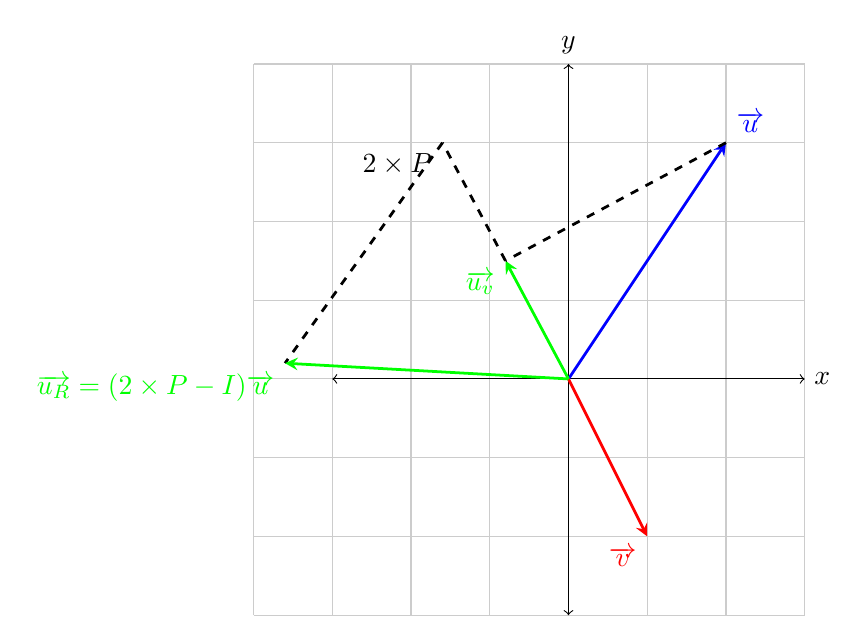
\begin{tikzpicture}
  \draw[thin,gray!40] (-4,-3) grid (3,4);
  \draw[<->] (-3,0)--(3,0) node[right]{$x$};
  \draw[<->] (0,-3)--(0,4) node[above]{$y$};
  \draw[line width=1pt,blue,-stealth](0,0)--(2, 3) node[anchor=south west]{$\boldsymbol{\overrightarrow{u}}$};
  \draw[line width=1pt,red,-stealth](0,0)--(1,-2) node[anchor=north east]{$\boldsymbol{\overrightarrow{v}}$};
  \draw[line width=1pt,green,-stealth](0,0)--(-0.8,1.5) node[anchor=north east]{$\boldsymbol{\overrightarrow{u_v}}$};
  \draw[line width=1pt,gray!200,dashed](2, 3) -- (-0.8,1.5){};
  \draw[line width=1pt,gray!200,dashed](-0.8,1.5)--(-1.6,3.0) node[anchor=north east]{$\boldsymbol{2 \times P}$};
  \draw[line width=1pt,gray!200,dashed](-1.6,3.0)--(-3.6,0.2) node[anchor=north east]{};
  \draw[line width=1pt,green,-stealth](0,0)--(-3.6,0.2) node[anchor=north east]{$\boldsymbol{\overrightarrow{u_R} = (2 \times P - I)\overrightarrow{u}}$};
\end{tikzpicture}

\section{Problème à résoudre}
Soit une base de données non triée à $N$ entrées. Nous voulons trouver un algorithme permettant de chercher efficacement un enregistrement dans cette base.


\subsection{Principe de l'algorithme}
L'algorithme de Grover permet de résoudre ce problème en quantique, en disposant de $N$ qubits intriqués pour calculer $2^N$ état 
(donc si on a $N$ entrées dans la base, il nous faut $log_2(N)$ qubits intriqués). Dans le cas de cet algorithme, on considère le problème suivant:
\medbreak
On marque $\{0, 1, 2, ..., N-1\}$ les enregistrements de la base de données, et on dénote $\omega$ l'état inconnu recherché. On dispose de la fonction suivante:

$f(x) = 
 \begin{cases}
   1, & \text{si x vérifie le critère} \; \omega \\
   0, & \text{sinon}
 \end{cases}
$

A la fin, on obtient un set de résultat. Or, lors de la mesure on va avoir au hasard une des solutions suivant les probabilités de chaque état, alors qu'on cherche
juste à savoir la (ou les) bonnes solutions. On rajoute donc une amplification d'amplitude permettant d'augmenter les probabilités des bons résultats et de diminuer
celles des mauvais.


\subsubsection*{Initialisation}

On commence avec :
$\ket{u_0} = (\ket{0}^{\bigotimes n}) \otimes \ket{1}$
: n-qubits à $\ket{0}$ et 1-qubit à $\ket{1}$

\subsubsection*{Etape 1}

On applique une porte de Hadamard à $\ket{u_0}$ pour avoir un état équiprobable:
$\ket{u_1} = H\ket{u_0} = \frac{1}{\sqrt{2^{n + 1}}}
\displaystyle\sum_{x=0}^{2^n-1} \ket{x}(\ket{0} - \ket{1})$

On pose alors $\ket{s} = \frac{1}{\sqrt{2^n}} \displaystyle\sum_{x=0}^{2^n-1} \ket{x}$

\subsubsection*{Etape 2: opérateurs de Grover}

On définit les deux opérateurs suivants:

$U_w = I - 2\ket{w}\bra{w}$, avec $w$ état cible correspondant à la solution du problème (amplitude de 1 sur l'état visé, amplitude nulle sur le reste)

$U_s = 2\ket{s}\bra{s} - I$

\begin{rem}
  On reconnait ici que ces deux opérateurs sont semblables à la reflection vue dans la partie 1.
\end{rem}

\paragraph*{Inversion d'amplitude}

L'opérateur $U_w$ effectue l'inversion de l'amplitude de l'état cible, tandis que l'opérateur $U_s$ effectue le miroir des amplitudes par rapport à la moyenne.

On applique $U_w$ puis $U_s$:

$U_w \ket{s} = (I - 2 \ket{w}\bra{w})\ket{s} \nonumber = \ket{s} - 2 \ket{w}\braket{w|s}$

Or, $\braket{w|s}$ est un produit scalaire. $\ket{w}$ est définit plus haut, et $\ket{s}$ est l'état équiprobable obtenu après la porte de hadamard. Le résultat est donc $\braket{w|s} = \frac{1}{\sqrt{2^n}}$. On peut donc réécrire:

$\ket{u_3} = U_w \ket{s} = \ket{s} - \frac{2}{\sqrt{2^n}}\ket{w}$

\paragraph*{Miroir à la moyenne}
On applique ensuite l'opérateur $U_s$ au résultat de $U_w$. On peut voir qu'en pratique $U_s$ effectue un miroir de $\ket{u_3}$ par rapport à $\ket{s}$.

\begin{align}
  U_s\ket{u_3} 
  &= (2\ket{s}\bra{s} - I)(\ket{s} - \frac{2}{\sqrt{2^n}}\ket{w}) \nonumber \\
  &= 2\ket{s}\braket{s|s} - \ket{s} - \frac{4}{\sqrt{2^n}} \ket{s} \braket{s|w} + \frac{2}{\sqrt{2^n}}\ket{w} \nonumber \\
  &= 2\ket{s} - \ket{s} + \frac{4}{\sqrt{2^n}} \times \frac{1}{\sqrt{2^n}} \ket{s} + \frac{2}{\sqrt{2^n}}\ket{w} \nonumber \\
  &= \ket{s} - \frac{4}{2^n} \ket{s} + \frac{2}{\sqrt{2^n}}\ket{w} \nonumber \\
  \ket{u_4}&=\frac{2^n - 4}{2^n}\ket{s} + \frac{2}{\sqrt{2^n}}\ket{w}
\end{align}
